\chapter{AAA model}

\section{Introduction}

AAA network security services provide the primary framework to set up access control on a network device. AAA is a way to control who is permitted to access a network (authenticate), what they can do while they are there (authorize), and to audit what actions they performed while accessing the network (accounting).\\

\textbf{Authentication:} Cisco provides two common methods of implementing AAA authentication: Local AAA Authentication and Server-Based AAA Authentication. \textbf{Local AAA Authentication} uses a local database for authentication. This method stores usernames and passwords locally in the Cisco router. With \textbf{Server-Based AAA Authentication}, the central AAA server contains the usernames and password for all users.\\

\textbf{Authorization} is typically implemented using a AAA server-based solution. Authorization uses a created set of attributes that describes the user’s access to the network. These attributes are compared to the information contained within the AAA database, and a determination of restrictions. Authorization is implemented immediately and automatically after the user is authenticated.\\

\textbf{Accounting} is implemented using a AAA server-based solution. This service reports usage statistics back to the ACS server. 

\section{Authentication}

\subsection{Local AAA authentication}

Local AAA Authentication should be configured for smaller networks. Smaller networks are those networks that have one or two routers that provide access to a limited number of users. This method uses the local usernames and passwords stored on a router. Configuring local AAA services to authenticate administrator access requires a few basic steps:

\begin{itemize}
  \item Add usernames and passwords to the local router database for users that need administrative access to the router.
  \item Enable AAA globally on the router.
  \item Configure AAA parameters on the router.
  \item Confirm and troubleshoot the AAA configuration.  
\end{itemize}

\begin{sexylisting}{Local AAA default authentication}
username ADMIN algorithm-type scrypt secret Str0ng5rPa55w0rd
username JR-ADMIN algorithm-type scrypt secret Str0ng5rPa55w0rd
aaa new-model
aaa authentication login default local-case
\end{sexylisting}

The above commands allow the ADMIN and JR-ADMIN users to log into the router via the console or vty terminal lines. The \code{default} keyword means that the authentication method applies to all lines. Alternatively, a custom authentication method (or named method) can be configured using \code{list-name}. Unlike \code{default} method, a named method has to be assigned to a particular line (console, aux, or virtual line) using \code{login auth <list-name>} command.\\ 

\begin{sexylisting}{Local AAA named authentication}
  username ADMIN algorithm-type scrypt secret Str0ng5rPa55w0rd
  username JR-ADMIN algorithm-type scrypt secret Str0ng5rPa55w0rd
  aaa new-model
  aaa authentication login SSH-LOGIN local-case
  line vty 0 4
  login auth SSH-LOGIN
  \end{sexylisting}

The final portion of the command identifies the type of methods that will be queried to authenticate the users. When a user attempts to log in, the first method listed is used. Cisco IOS software attempts the second authentication method only when there is no response or an error from the first method occurs. This process continues until no other authentication methods are available.

\subsection{Server-based AAA authentication}

% Before enabling AAA, at least a local database entry must be configured. To enable AAA, the \code{aaa new-model} global configuration command must \emph{first} be configured. No other AAA commands are available until this command is entered.\\

% Create the default login authentication list by issuing the \code{authentication login default method1[method2][method3]} command. The following commands configure the list to first use RADIUS (\code{group radius}) for the authentication service, and then none. The keyword \code{none} means that if no RADIUS server can be reached and authentication cannot be performed, the router globally allows access without authentication. This is a safeguard measure in case the router starts up without connectivity to an active RADIUS server.\\

% The \code{aaa authentication login default} command allows the HUY users to log into the router vty terminal lines. The \code{default} keyword means that the authentication method applies to all lines (vty, console, aux). However, if you want AAA authentication only applied to vty line, replace \code{default} by the name of the method list, for example \code{SSH-LOGIN}.

\begin{sexylisting}{Default server-based AAA authentication}
username HUY algorithm-type scrypt secret cisco12345

aaa new-model
aaa authentication login default group radius none

aaa local authentication attempts max-fail 3
\end{sexylisting}

\begin{sexylisting}{Custom server-based AAA authentication}
username HUY algorithm-type scrypt secret cisco12345

aaa new-model
aaa authentication login SSH-LOGIN group radius none

line vty 0 4
login authentication SSH-LOGIN

aaa local authentication attempts max-fail 3
\end{sexylisting}


Below is the syntax of \code{aaa authentication login} command. This command lists authentication methods (four methods at the maximum) in the order of execution. In other words, the next listed authentication method is executed only when there is no response or an error from the previous method occurs. The name of this list is specified by the user as \code{<list-name>}. Table \ref{login} shows the command syntax and all available method type keywords.

\tableStart[\caption{AAA login authentication methods}\label{login}] {|l|l|} 
\multicolumn{2}{|c|}{\code{aaa authentication login {default | list-name} method1 ... method4}}\w
\head{Keywords} & \head{Description} \w
\code{enable} & Use the enable password\w
\code{local} & Use local username database\w
\code{local-case} & Use case-sensitive local username database\w
\code{none} & Ensure that the authentication succeeds even if all methods return an error \w
\code{group radius} & Use the lists of all RADIUS servers \w
\code{group tacacs+} & Use the lists of all TACACS+ servers \w
\code{group <group-name>} & Use a subset of RADIUS or TACACS+ servers \w
\tableEnd

The \code{aaa local authentication attempts max-fail} command locks the user account if the authentication fails. The locked out user account remains locked until it is manually cleared by an administrator using the \code{clear aaa local user lockout} privileged EXEC mode command. This command is different from \code{login delay} command, which introduces a delay between failed login attempts without locking the account.\\

To display a list of all locked-out users, use the \code{sh aaa local user lockout} command. To display the history of activities (attributes), use the \code{sh aaa user} command. This command does not provide information for all users who are logged into a device, but only for those who have been authenticated or authorized using AAA, or whose sessions are being accounted for by the AAA module. The \code{sh aaa sessions} command can be used to show the unique ID of a session. The \code{debug aaa authentication} command is instrumental when troubleshooting AAA problems. 

\subsection{Server-based AAA authentication}

\subsection{RADIUS vs TACACS+}

The Cisco Secure Access Control System (ACS) is a centralized solution that ties together an enterprise’s network access policy and identity strategy. Cisco Secure ACS supports both TACACS+ and RADIUS protocols (Table \ref{ACS}).

\tableStart[\caption{TACACS+ and RADIUS protocols}\label{ACS}] {|p{5\xm}|p{5\xm}|} 
\head{TACACS+} & \head{RADIUS} \\
\hline

Separates authentication and authorization & Combines RADIUS authentication and authorization as one process.\w
Encrypts all communication & Encrypts only the password using MD5 \\\hline
TCP port 49 & UDP port 1645 or 1812 for authentication, UDP port 1646 or 1813 for accounting\\\hline
Multiprotocol support & Supports remote-access technologies, VoIP, 802.1X, and Session Initiation Protocol (SIP) \w

\tableEnd

\note A next-generation AAA protocol alternative to RADIUS is the DIAMETER AAA protocol.\\

\textbf{Microsoft Active Directory (AD)} is a directory service for Windows domain networks, and is part of most Windows Server operating systems. The AD domain controller is used to enforce security policies by authenticating and authorizing users when they log into the Windows domain. \textbf{Cisco Secure ACS} can be integrated to use the AD service. It supports both TACACS+ and RADIUS. Instead of Cisco Secure ACS, Windows Server can also be configured as a AAA server using RADIUS, known as \textbf{NPS (Network Policy Server)}.

\subsection{Identity Services Engine (ISE)}

Cisco Identity Services Engine (ISE) is an identity and access control policy platform that enables enterprises to enforce compliance (including \emph{BYOD}), enhance infrastructure security, and streamline their service operations. The architecture of this engine allows administrator to gather real-time information to make proactive governance decisions by tying identity to various network elements. Cisco ISE combines policy definition, control, and reporting in \emph{one} appliance.\\

Cisco ISE is the main policy component for \textbf{Cisco TrustSec}, which protects end devices from unauthorized access. There are four features in the ISE toolset: AAA, Device profiling, Posture assessment, and Guest assessment.

\subsection{Configuration}

There are three basic steps to configure server-based authentication:

\begin{enumerate}
\item Globally enable AAA
\item Specify the Cisco Secure ACS (TACACS+ or RADIUS server) and Configure the encryption key between the server and router.
\item Configure the AAA authentication method list to refer to the TACACS+ or RADIUS server. For redundancy, it is possible to configure more than one server.
\end{enumerate}

The following commands show how to accomplish step 1 and 2:

\begin{sexylisting}{Create a TACACS+ server}
aaa new-models

tacacs server Server-T
  address ipv4 192.168.1.101
  single-connection
  key TACACS-Pa55w0rd
\end{sexylisting}

\begin{sexylisting}{Create a RAIDUS server}
aaa new-models
 
radius server Server-R
  address ipv4 192.168.1.101 auth-port 1812 acct-port 1813
  single-connection
  key RADIUS-Pa55w0rd
\end{sexylisting}

The \code{address ipv4} command allows the option to modify IPv4 address of the server, authentication port, and accounting port. The \code{key} command is used to configure the shared secret key, which must be exactly the same way on both the router and the server.\\

The \code{single-connection} command (TACACS+ only) maintains a single TCP connection for the life of the session. Otherwise, by default, a TCP connection is opened and closed for each session. Because RADIUS uses UDP, there is no \code{single-connection} keyword.\\

When the AAA servers have been identified as shown in the above commands, the servers must be included in the method list of the \code{aaa authentication login} command. AAA servers are identified using the \code{group tacacs+} or \code{group radius} keywords. 

\begin{sexylisting}{Configure Authentication to Use the AAA Server}
aaa authentication login default group tacacs+ group radius local-base
\end{sexylisting}

The above commands configure a method list for the default login to authenticate first using a TACACS+ server, second with a RADIUS server, and finally with a local username database. It is important to realize that R1 will only attempt to authenticate using RADIUS if the TACACS+ server is not reachable. Likewise, R1 would only attempt to authenticate using the local database if the TACACS+ and RADIUS servers are unavailable.\\

Troubleshoot Server-based AAA authentication using the following commands: \code{debug radius}, \code{debug tacacs}, \code{debug tacacs events}, and \code{debug aaa authentication}.

\section{Server-based AAA authorization}

When AAA authorization is not enabled, all users are allowed full access. After authentication is started, the default changes to allow no access. This means that the administrator must create a user with full access rights before authorization is enabled. \\

To configure command authorization, use the \code{aaa authorization} command. The service type can specify the types of commands or services:
\code{network} -- For network services such as PPP, \code{exec} -- For starting an exec (shell), \code{commands <level>} -- For exec (shell) commands. 

\begin{sexylisting}{AAA Authorization Configuration}
aaa authorization {network | commands <level> | exec} {default | <list-name>} 
  method1 ... method4
  
aaa authorization exec default group tacacs+
\end{sexylisting}

\section{Server-based AAA accounting}

To configure AAA accounting, use the \code{aaa accounting} command. 

\begin{sexylisting}{AAA Authorization Configuration}
aaa accounting {network | connection | exec} {default | <list-name>} 
         {statrt-stop | stop-only | none} [broadcast] method1 ... method4

aaa account exec default start-stop group tacacs+
\end{sexylisting}

The following three parameters are commonly used aaa accounting keywords:

\begin{itemize}
\item \code{network} - Runs accounting for all network-related service requests, including PPP.
\item \code{exec} - Runs accounting for the EXEC shell session.
\item \code{connection} - Runs accounting on all outbound connections such as SSH and Telnet.
\end{itemize}

Next, the record type, or trigger, is configured. The trigger specifies what actions cause accounting records to be updated. Possible triggers include:

\begin{itemize}
\item \code{start-stop} - Sends a "start" accounting notice at the beginning of a process and a "stop" accounting notice at the end of a process.
\item \code{stop-only} - Sends a "stop" accounting record for all cases including authentication failures.
\item \code{none} - Disables accounting services on a line or interface.
\end{itemize}
    

\section{802.1X Port-Based Authentication}

\subsection{Operation}

The IEEE 802.1X standard defines a port-based access control and authentication protocol that restricts unauthorized devices from connecting to a LAN through publicly accessible switch ports. Figure \ref{802.1X} shows that with 802.1X port-based authentication roles:

\begin{itemize}
\item \textbf{Supplicant (Client)} -- The device that requests access to LAN. The workstation must be running 802.1X-compliant client software. 
\item \textbf{Authenticator (Switch)} -- Controls physical access to the network based on the authentication status of the client. The switch acts as an intermediary (proxy) between the supplicants and the authentication server. It verifies information from the client and relays a response to the client. The switch uses a RADIUS software agent, which is responsible for encapsulating and de-encapsulating the EAP frames and interacting with the authentication server.
\item \textbf{Authentication server} -- Performs the actual authentication of the client. The authentication server validates the identity of the client and notifies the switch. Because the switch acts as the proxy, the authentication service is transparent to the client. The RADIUS security system with EAP extensions is the only supported authentication server.
\end{itemize}

\begin{figure}[hbtp]
\caption{802.1X roles}\label{802.1X}
\centering
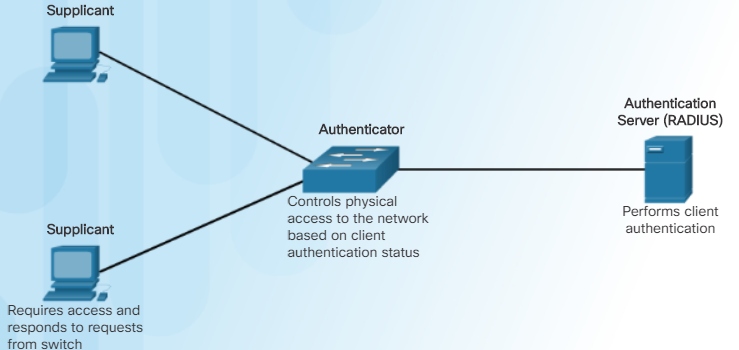
\includegraphics[scale=0.7]{pictures/8021X.PNG}
\end{figure}

If the Supplicant is successfully authenticated (receives an Accept frame from the authentication server), the port state changes to authorized, and all frames from the authenticated client are allowed through the port. If the authentication fails, the port remains in the unauthorized state, but authentication can be retried. If the authentication server cannot be reached, the switch can resend the request. If no response is received from the server after the specified number of attempts, authentication fails, and network access is not granted.

\begin{figure}[hbtp]
\caption{802.1X message exchange}\label{MessageExchange}
\centering
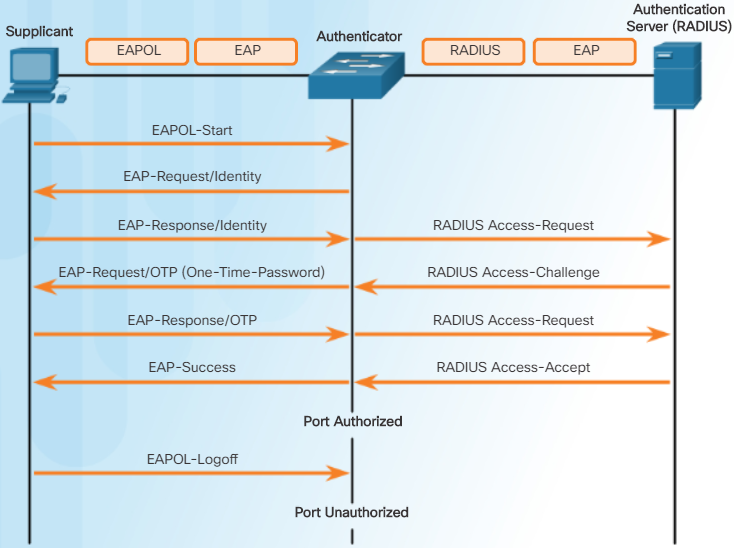
\includegraphics[scale=0.7]{pictures/MessageExchange.PNG}
\end{figure}

\paragraph{Message exchange} Until the workstation is authenticated, 802.1X access control enables only EAPOL (EAP over LAN) traffic through the port to which the workstation is connected. After authentication succeeds, normal traffic can pass through the port. Figure \ref{MessageExchange} shows the complete message exchange between the supplicant, authenticator, and the authentication server. The encapsulation occurs as follows:

\begin{itemize}
\item Between the supplicant and the authenticator - EAP data is encapsulated in EAPOL frames.
\item Between the authenticator and the authentication server - EAP data is encapsulated using RADIUS.
\end{itemize}

\subsection{Port Authorization State}

When configured for 802.1X port-based authentication, the port starts in the \emph{unauthorized state}. While in this state, the port disallows all ingress and egress traffic except for 802.1X protocol packets. When a client is successfully authenticated, the port transitions to the \emph{authorized state}, allowing all traffic for the client to flow normally. \\

When a client logs out, it sends an EAPOL-logout message, causing the switch port to transition to the unauthorized state. If the link state of a port changes from up to down, or if an EAPOL-logoff frame is received, the port returns to the unauthorized state.\\    

If the supplicant does not support 802.1X, the port remains in the unauthorized state. In contrast, if a switch that is not running the 802.1X protocol, the client begins sending frames as if the port is in the authorized state.\\


\subsection{Configuration}

The following commands show a scenario where a PC is attached to F0/1 on the switch and the device is getting authenticated via 802.1X with a RADIUS server. Configuring 802.1X requires a few basic steps:



\begin{sexylisting}{802.1X configuration}
aaa new-models

radius server Server-R
  address ipv4 192.168.1.101 auth-port 1812 acct-port 1813
  single-connection
  key RADIUS-Pa55w0rd
  exit
 
aaa authentication dot1x default group radius
dot1x system-auth-control

interface f0/1
  sw mode access
  authentication port-control auto
  dot1x pae authenticator
  exit
\end{sexylisting}

\begin{enumerate}
\item Enable AAA 
\item Configure a RADIUS server
\item Create an 802.1X port-based authentication method list using the \code{aaa authentication dot1x} command.
\item Globally enable 802.1X port-based authentication using the \code{dot1x system-auth-control} command.
\item Enable port-based authentication on the interface using the \code{authentication port-control auto} command.
\item Enable 802.1X authentication on the interface using the \code{dot1x pae} command. The \code{authenticator} options sets the Port Access Entity (PAE) type so the interface acts only as an authenticator and will not respond to any messages meant for a supplicant.
\end{enumerate}

The \code{authentication port-control} command has three options for port state:

\begin{itemize}
\item \code{auto} -- Enable 802.1X authentication
\item \code{force-authorized} -- Disable 802.1X authentication. This option causes the port to remain authorized and transmit normal traffic. By default, a port is in the force-authorized state.
\item \code{force-unauthorized} -- This option causes the port to remain unauthorized and lock all authentication services.
\end{itemize}